%==============================================================================
% EECS 127 - Lecture 3: Fundamental Theorem of Linear Algebra
%==============================================================================

\documentclass[10pt, twocolumn]{article}
\usepackage[margin=0.75in, columnsep=0.3in]{geometry}

%------------------------------------------------------------------------------
% REQUIRED PACKAGES
%------------------------------------------------------------------------------
\usepackage{amsmath, amssymb, amsthm}
\usepackage{microtype}
\usepackage{enumitem}
\usepackage{fancyhdr}
\usepackage{titlesec}
\usepackage{tcolorbox}
\usepackage{booktabs}
\usepackage{tikz}
\usetikzlibrary{positioning, arrows.meta, calc}

%------------------------------------------------------------------------------
% SPACING
%------------------------------------------------------------------------------
\linespread{1.08}
\setlength{\parskip}{0.4ex plus 0.2ex minus 0.1ex}

%------------------------------------------------------------------------------
% BOX STYLES
%------------------------------------------------------------------------------
\tcbset{
    boxrule=0.8pt,
    colback=white,
    colframe=black,
    arc=0pt,
    boxsep=3pt,
    left=4pt, right=4pt, top=4pt, bottom=4pt
}

\newtcolorbox{result}{
    boxrule=0pt,
    colback=black!5,
    colframe=white,
    arc=0pt,
    boxsep=2pt,
    left=4pt, right=4pt, top=4pt, bottom=4pt
}

%------------------------------------------------------------------------------
% SECTION FORMATTING
%------------------------------------------------------------------------------
\titleformat{\section}{\large\bfseries}{\thesection.}{0.5em}{}
\titleformat{\subsection}{\normalsize\bfseries}{\thesubsection}{0.5em}{}
\titlespacing*{\section}{0pt}{1.5ex}{1ex}
\titlespacing*{\subsection}{0pt}{1ex}{0.5ex}

%------------------------------------------------------------------------------
% LIST FORMATTING
%------------------------------------------------------------------------------
\setlist{itemsep=1pt, topsep=3pt, parsep=1pt, leftmargin=1.5em}

%------------------------------------------------------------------------------
% HEADER/FOOTER
%------------------------------------------------------------------------------
\pagestyle{fancy}
\fancyhf{}
\fancyhead[L]{\small EECS 127}
\fancyhead[R]{\small Lecture 3}
\fancyfoot[C]{\small\thepage}
\renewcommand{\headrulewidth}{0.4pt}

%------------------------------------------------------------------------------
% THEOREM ENVIRONMENTS
%------------------------------------------------------------------------------
\theoremstyle{definition}
\newtheorem{definition}{Definition}
\newtheorem{example}{Example}

\theoremstyle{plain}
\newtheorem{theorem}{Theorem}
\newtheorem{lemma}{Lemma}

%------------------------------------------------------------------------------
% CUSTOM COMMANDS
%------------------------------------------------------------------------------
\newcommand{\RR}{\mathbb{R}}
\newcommand{\NN}{\mathcal{N}}
\newcommand{\Range}{\mathcal{R}}
\DeclareMathOperator{\rank}{rank}
\DeclareMathOperator{\spn}{span}

%==============================================================================

\begin{document}

\noindent
\begin{minipage}{\linewidth}
    \centering
    \textbf{\Large Lecture 3: Fundamental Theorem of Linear Algebra} \\[0.5em]
    \hrule
\end{minipage}
\vspace{1em}

%==============================================================================
\section{Orthogonal Decomposition of Space}
%==============================================================================

Any finite-dimensional inner product space decomposes into two orthogonal pieces. \textbf{Why care?} This decomposition underpins least squares, projections, and the structure of linear systems. When $Ax = b$ has no exact solution, orthogonal decomposition reveals the best approximation.

We first make precise what ``orthogonal pieces'' means.

\begin{definition}[Orthogonal Complement]
For a subspace $S$ of an inner product space $X$, the \textbf{orthogonal complement} is
\[
    S^\perp = \{x \in X : \langle x, s \rangle = 0 \text{ for all } s \in S\}
\]
\end{definition}

\begin{lemma}[Basis Test for Orthogonality]\label{lem:basis-test}
Let $S \subseteq X$ have basis $\{s_1, \ldots, s_k\}$. Then $x \in S^\perp$ iff $\langle x, s_i \rangle = 0$ for $i = 1, \ldots, k$.
\end{lemma}

\begin{proof}
($\Rightarrow$) If $x \in S^\perp$, then $\langle x, s \rangle = 0$ for all $s \in S$; in particular, $\langle x, s_i \rangle = 0$ for each basis vector.

($\Leftarrow$) Suppose $\langle x, s_i \rangle = 0$ for all $i$. Any $s \in S$ can be written $s = \sum_{i=1}^k \alpha_i s_i$. By linearity:
\[
\langle x, s \rangle = \sum_{i=1}^k \alpha_i \langle x, s_i \rangle = 0
\]
Thus $x \in S^\perp$.
\end{proof}

\begin{tcolorbox}[colframe=black!50, title={\small Practical Implication}]
To verify $x \in S^\perp$, check orthogonality to a \emph{basis} of $S$, not every vector. Infinitely many conditions reduce to finitely many.
\end{tcolorbox}

\begin{definition}[Direct Sum]
The \textbf{direct sum} $X = S \oplus S^\perp$ means:
\begin{enumerate}[label=(\roman*)]
    \item \textbf{Existence:} Every $x \in X$ can be written as $x = s + s^\perp$ with $s \in S$, $s^\perp \in S^\perp$.
    \item \textbf{Uniqueness:} The decomposition is unique.
\end{enumerate}
Equivalently: $S + S^\perp = X$ and $S \cap S^\perp = \{0\}$.
\end{definition}

\begin{tcolorbox}[colframe=black!50, title={\small Why Uniqueness Follows from $S \cap S^\perp = \{0\}$}]
If $s_1 + s_1^\perp = s_2 + s_2^\perp$, then $s_1 - s_2 = s_2^\perp - s_1^\perp$. The LHS is in $S$; the RHS is in $S^\perp$. Thus both sides lie in $S \cap S^\perp = \{0\}$, so $s_1 = s_2$.
\end{tcolorbox}

\begin{theorem}[Orthogonal Decomposition]
For any subspace $S$ of a finite-dimensional inner product space $X$:
\[
    X = S \oplus S^\perp
\]
Moreover, $\dim(S) + \dim(S^\perp) = \dim(X)$.
\end{theorem}

\begin{proof}
\textbf{Step 1: $S \cap S^\perp = \{0\}$.} If $v \in S \cap S^\perp$, then $\langle v, v \rangle = 0$. By positive definiteness, $v = 0$.

\textbf{Step 2: Existence.} Let $\{s_1, \ldots, s_k\}$ be an orthonormal basis for $S$ (obtained via Gram--Schmidt). For any $x \in X$, define:
\[
s = \sum_{i=1}^k \langle x, s_i \rangle s_i \in S, \qquad s^\perp = x - s
\]
Then $\langle s^\perp, s_j \rangle = \langle x, s_j \rangle - \langle x, s_j \rangle = 0$ using orthonormality $\langle s_i, s_j \rangle = \delta_{ij}$. By Lemma~\ref{lem:basis-test}, $s^\perp \in S^\perp$.

\textbf{Step 3: Dimension.} From Step 2, $X = S + S^\perp$. Combined with Step 1 ($S \cap S^\perp = \{0\}$), we have $X = S \oplus S^\perp$. Thus:
\[
\dim(X) = \dim(S) + \dim(S^\perp)
\]
\end{proof}

\begin{tcolorbox}[colframe=black!50, title={\small Geometric Intuition}]
In $\RR^3$: if $S$ is a plane through the origin, then $S^\perp$ is the perpendicular line. Every vector splits into a plane component plus a line component---orthogonal pieces summing to the original.
\end{tcolorbox}

\begin{example}[Orthogonal Decomposition in $\RR^2$]
Let $S = \text{span}\{(1,0)\}$ be the $x$-axis in $\RR^2$. Then:
\[
    S^\perp = \text{span}\{(0,1)\} \quad \text{(the $y$-axis)}
\]
Any vector $(a, b) \in \RR^2$ decomposes as:
\[
    \underbrace{(a, b)}_{\in \RR^2} = \underbrace{(a, 0)}_{\in S} + \underbrace{(0, b)}_{\in S^\perp}
\]
Notice that $(a,0) \cdot (0,b) = 0$, confirming orthogonality.
\end{example}

We now turn to how matrices decompose $\RR^n$ and $\RR^m$ into orthogonal pieces.

%==============================================================================
\section{Four Fundamental Subspaces}
%==============================================================================

A matrix $A \in \RR^{m \times n}$ has four fundamental subspaces. \textbf{Why four?} $A$ maps $\RR^n \to \RR^m$, creating two complementary subspaces in each space.

\begin{center}
\begin{tabular}{@{}llll@{}}
\toprule
\textbf{Subspace} & \textbf{Name} & \textbf{Lives in} & \textbf{Dimension} \\
\midrule
$\NN(A)$ & Null space & $\RR^n$ & $n - r$ \\
$\Range(A^\top)$ & Row space & $\RR^n$ & $r$ \\
$\Range(A)$ & Column space & $\RR^m$ & $r$ \\
$\NN(A^\top)$ & Left null space & $\RR^m$ & $m - r$ \\
\bottomrule
\end{tabular}
\end{center}
Here $r = \text{rank}(A)$.

\begin{tcolorbox}[colframe=black!50, title={\small Dimension Check}]
In $\RR^n$: $(n-r) + r = n$. In $\RR^m$: $r + (m-r) = m$. (Rank-Nullity Theorem.)
\end{tcolorbox}

% TikZ diagram of the four fundamental subspaces
\begin{center}
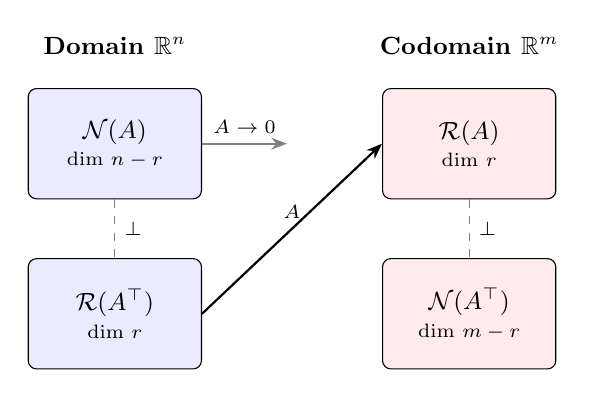
\begin{tikzpicture}[
    space/.style={draw, rounded corners=3pt, minimum width=2.2cm, minimum height=1.4cm, align=center, font=\small},
    arrow/.style={-{Stealth[length=2mm]}, thick},
    ortho/.style={dashed, gray},
    scale=0.9
]
% Domain R^n
\node[space, fill=blue!8] (null) at (0,1.2) {$\NN(A)$\\[-1pt]{\scriptsize dim $n-r$}};
\node[space, fill=blue!8] (row) at (0,-1.2) {$\Range(A^\top)$\\[-1pt]{\scriptsize dim $r$}};
\node[above=0.3cm of null, font=\small\bfseries] {Domain $\RR^n$};

% Codomain R^m
\node[space, fill=red!8] (col) at (5,1.2) {$\Range(A)$\\[-1pt]{\scriptsize dim $r$}};
\node[space, fill=red!8] (leftnull) at (5,-1.2) {$\NN(A^\top)$\\[-1pt]{\scriptsize dim $m-r$}};
\node[above=0.3cm of col, font=\small\bfseries] {Codomain $\RR^m$};

% Orthogonality markers
\draw[ortho] (null.south) -- node[right, font=\scriptsize, black] {$\perp$} (row.north);
\draw[ortho] (col.south) -- node[right, font=\scriptsize, black] {$\perp$} (leftnull.north);

% Mapping arrows
\draw[arrow] (row.east) -- node[above, font=\scriptsize] {$A$} (col.west);
\draw[arrow, gray] (null.east) -- node[above, font=\scriptsize, black] {$A \to 0$} ++(1.2,0);
\end{tikzpicture}
\end{center}

\subsection{Definitions and Significance}

\textbf{Null space} (kernel): $\NN(A) = \{x \in \RR^n : Ax = 0\}$. Captures information loss: if $x_1 - x_2 \in \NN(A)$, then $Ax_1 = Ax_2$.

\textbf{Column space} (range): $\Range(A) = \{Ax : x \in \RR^n\}$. All possible outputs. $Ax = b$ is solvable iff $b \in \Range(A)$.

\textbf{Row space}: $\Range(A^\top) = \{A^\top y : y \in \RR^m\}$. Orthogonal to the null space; represents directions $A$ can detect.

\textbf{Left null space}: $\NN(A^\top) = \{y \in \RR^m : A^\top y = 0\}$. When $Ax = b$ has no solution, the component of $b$ in $\NN(A^\top)$ measures the residual.

\subsection{Example: A $2 \times 3$ Matrix}

\begin{example}
Consider $A = \begin{pmatrix} 1 & 2 & 3 \\ 2 & 4 & 6 \end{pmatrix} \in \RR^{2 \times 3}$. Row 2 equals $2 \times$ row 1, so $\text{rank}(A) = 1$.

\textbf{Step 1: Null space $\NN(A) \subseteq \RR^3$.} Solve $Ax = 0$: both rows give $x_1 + 2x_2 + 3x_3 = 0$, so $x_1 = -2x_2 - 3x_3$:
\[
    \NN(A) = \text{span}\left\{ \begin{pmatrix} -2 \\ 1 \\ 0 \end{pmatrix}, \begin{pmatrix} -3 \\ 0 \\ 1 \end{pmatrix} \right\} \quad (\dim = 2 = n - r)
\]

\textbf{Step 2: Row space $\Range(A^\top) \subseteq \RR^3$.} Spanned by rows of $A$:
\[
    \Range(A^\top) = \text{span}\left\{ \begin{pmatrix} 1 \\ 2 \\ 3 \end{pmatrix} \right\} \quad (\dim = 1 = r)
\]

\textbf{Step 3: Verify orthogonality.} $(1,2,3) \cdot (-2,1,0) = 0$ \checkmark\quad and $(1,2,3) \cdot (-3,0,1) = 0$ \checkmark

\textbf{Step 4: Column space $\Range(A) \subseteq \RR^2$.} All columns are multiples of $(1,2)^\top$:
\[
    \Range(A) = \text{span}\left\{ \begin{pmatrix} 1 \\ 2 \end{pmatrix} \right\} \quad (\dim = 1 = r)
\]

\textbf{Step 5: Left null space $\NN(A^\top) \subseteq \RR^2$.} Solve $A^\top y = 0$: all rows give $y_1 + 2y_2 = 0$:
\[
    \NN(A^\top) = \text{span}\left\{ \begin{pmatrix} -2 \\ 1 \end{pmatrix} \right\} \quad (\dim = 1 = m - r)
\]

\textbf{Step 6: Verify.} $(1,2) \cdot (-2,1) = 0$ \checkmark\quad Column space $\perp$ left null space.
\end{example}

\begin{tcolorbox}[colframe=black!50, title={\small Summary}]
For $A \in \RR^{2 \times 3}$ with rank 1: In $\RR^3$, $\NN(A)$ (dim 2) $\perp$ $\Range(A^\top)$ (dim 1). In $\RR^2$, $\NN(A^\top)$ (dim 1) $\perp$ $\Range(A)$ (dim 1). Dimensions always sum to ambient space dimension.
\end{tcolorbox}

We now prove \emph{why} these orthogonality relationships hold.

%==============================================================================
\section{Fundamental Orthogonal Decompositions}
%==============================================================================

The four subspaces form orthogonal pairs: a consequence of the adjoint relationship between $A$ and $A^\top$.

\begin{lemma}[Adjoint Identity]\label{lem:transpose-ip}
For $A \in \RR^{m \times n}$, $x \in \RR^n$, $y \in \RR^m$: \ $\langle A^\top y, x \rangle = \langle y, Ax \rangle$.
\end{lemma}

\begin{proof}
$\langle A^\top y, x \rangle = (A^\top y)^\top x = y^\top A x = \langle y, Ax \rangle$.
\end{proof}

\textit{Remark:} This identity underlies both orthogonality relations. $A$ and $A^\top$ are adjoint operators.

\begin{result}
\textbf{Fundamental Theorem of Linear Algebra:}
\[
    \NN(A) \oplus \Range(A^\top) = \RR^n
\]
\[
    \NN(A^\top) \oplus \Range(A) = \RR^m
\]
\end{result}

Every $x \in \RR^n$ uniquely decomposes into null space and row space components; every $y \in \RR^m$ splits into column space and left null space components. Equivalently:
\begin{result}
\[
    \NN(A) = \Range(A^\top)^\perp \quad \text{and} \quad \NN(A^\top) = \Range(A)^\perp
\]
\end{result}

\begin{tcolorbox}[colframe=black!50, title={\small Applications}]
\textbf{Least Squares:} When $b \notin \Range(A)$, decompose $b = b_{\parallel} + b_\perp$ with $b_{\parallel} \in \Range(A)$ and $b_\perp \in \NN(A^\top)$. The least squares solution solves $Ax = b_{\parallel}$.

\textbf{Rank-Nullity:} The decomposition implies $\dim(\NN(A)) + \text{rank}(A) = n$.
\end{tcolorbox}

%==============================================================================
\section{Proof: $\NN(A) = \Range(A^\top)^\perp$}
%==============================================================================

We prove one orthogonality relation; the other follows by applying the same argument to $A^\top$.

\begin{tcolorbox}[colframe=black!50, title={\small Proof Strategy: Double Inclusion}]
To prove $X = Y$: show (a) $X \subseteq Y$ and (b) $Y \subseteq X$. Here $X = \NN(A)$, $Y = \Range(A^\top)^\perp$.
\end{tcolorbox}

\subsection{Part (a): $\NN(A) \subseteq \Range(A^\top)^\perp$}

\textbf{Goal:} Every null space vector is orthogonal to every row space vector.

\textbf{Step 1:} Take $x \in \NN(A)$, so $Ax = 0$. For any $w \in \Range(A^\top)$, write $w = A^\top z$ for some $z \in \RR^m$.

\textbf{Step 2:} Apply Lemma~\ref{lem:transpose-ip}:
\[
    \langle w, x \rangle = \langle A^\top z, x \rangle = \langle z, Ax \rangle = \langle z, 0 \rangle = 0
\]

\textbf{Step 3:} Since $w$ was arbitrary, $x \in \Range(A^\top)^\perp$.

\subsection{Part (b): $\Range(A^\top)^\perp \subseteq \NN(A)$}

\textbf{Goal:} Any vector orthogonal to the row space lies in the null space.

\textbf{Step 1:} Take $x \in \Range(A^\top)^\perp$, so $\langle x, w \rangle = 0$ for all $w \in \Range(A^\top)$.

\textbf{Step 2:} In particular, for all $z \in \RR^m$:
\[
    0 = \langle x, A^\top z \rangle = \langle A^\top z, x \rangle = \langle z, Ax \rangle
\]
where the last step uses Lemma~\ref{lem:transpose-ip}.

\textbf{Step 3:} Since $\langle Ax, z \rangle = 0$ for all $z$, choosing $z = Ax$ gives $\|Ax\|^2 = 0$, hence $Ax = 0$.

\begin{tcolorbox}[colframe=black!50, title={\small The Finishing Move: Why This Works}]
If $\langle v, z \rangle = 0$ for \emph{all} $z \in \RR^m$, then $v = 0$. Why?

\textbf{Method 1:} Choose $z = e_i$ (standard basis): $\langle v, e_i \rangle = v_i = 0$ for each $i$. Every component vanishes, so $v = 0$.

\textbf{Method 2:} Choose $z = v$ to get $\|v\|^2 = 0$, hence $v = 0$.
\end{tcolorbox}

\subsection{Completing the Proof}

Both inclusions give $\NN(A) = \Range(A^\top)^\perp$, equivalent to $\NN(A) \oplus \Range(A^\top) = \RR^n$. $\square$

\begin{tcolorbox}[colframe=black!50, title={\small Corollary: Rank-Nullity}]
From $\NN(A) = \Range(A^\top)^\perp$: $\dim(\NN(A)) = n - \dim(\Range(A^\top)) = n - r$. The Fundamental Theorem implies Rank-Nullity.
\end{tcolorbox}

\begin{tcolorbox}[colframe=black!50, title={\small Intuition}]
Each row $a_i^\top$ of $A$ gives an equation $a_i^\top x = 0$: ``$x$ is orthogonal to $a_i$.'' To satisfy $Ax = 0$, $x$ must be orthogonal to every row, hence to their span (the row space).
\end{tcolorbox}

%==============================================================================
\section{The Generalized Proof Method}
%==============================================================================

\begin{tcolorbox}[colframe=black!50, title={\small Key Insight}]
The proof of $\NN(A) = \Range(A^\top)^\perp$ is not just a result---it's a \textbf{reusable template} for proving orthogonality relationships throughout linear algebra.
\end{tcolorbox}

\subsection{The Six-Step Template}

\begin{enumerate}
    \item \textbf{Reduce to two inclusions.} To prove $S = T$, show $S \subseteq T$ and $T \subseteq S$ separately.

    \item \textbf{Start with arbitrary element.} Begin each direction with ``Let $x \in S$'' (or $T$). This is the only starting point.

    \item \textbf{Translate orthogonal complement.} Use the ``dictionary'': $x \in S^\perp$ means $\langle x, w \rangle = 0$ for all $w \in S$.

    \item \textbf{Replace subspace elements.} If $w \in \Range(A^\top)$, write $w = A^\top z$ for some $z$. If $w \in \Range(A)$, write $w = Ax$.

    \item \textbf{Apply the adjoint identity.} The ``bridge'' between null space and range: $\langle A^\top y, x \rangle = \langle y, Ax \rangle$.

    \item \textbf{Use the finishing move.} ``Orthogonal to everything $\Rightarrow$ zero'': if $\langle v, z \rangle = 0$ for all $z$, then $v = 0$ (choose $z = v$).
\end{enumerate}

\begin{tcolorbox}[colframe=black!50, title={\small One-Line Summary}]
\textbf{Unpack} $\to$ \textbf{Rewrite} $\to$ \textbf{Transpose} $\to$ \textbf{Zero} $\to$ \textbf{Conclude}
\end{tcolorbox}

\begin{tcolorbox}[colframe=black!50, title={\small Where This Method Applies}]
\begin{itemize}
    \item Proving $\NN(A^\top) = \Range(A)^\perp$ (Section 5)
    \item Deriving the normal equations for least squares
    \item Showing projection matrices satisfy $P^2 = P$
    \item Proving optimality conditions in constrained optimization
\end{itemize}
\end{tcolorbox}

%==============================================================================
\section{Sketch: $\NN(A^\top) = \Range(A)^\perp$}
%==============================================================================

For completeness, we outline the analogous proof.

\textbf{Part (a): $\NN(A^\top) \subseteq \Range(A)^\perp$.} Let $y \in \NN(A^\top)$. For any $w = Ax \in \Range(A)$:
\[
\langle y, w \rangle = \langle y, Ax \rangle = (A^\top y)^\top x = 0
\]

\textbf{Part (b): $\Range(A)^\perp \subseteq \NN(A^\top)$.} Let $y \in \Range(A)^\perp$. Then $\langle y, Ax \rangle = 0$ for all $x$, so $\langle A^\top y, x \rangle = 0$ for all $x$. Choosing $x = A^\top y$ gives $A^\top y = 0$. $\square$

%==============================================================================
\section{Application: Minimum-Norm Solutions}
%==============================================================================

The FTLA has immediate applications to optimization. Consider \emph{underdetermined} systems where infinitely many solutions exist.

\begin{tcolorbox}[colframe=black!50, title={\small Problem: Minimum-Norm Solution}]
Given $A \in \RR^{m \times n}$ with $m < n$ and full row rank, and $b \in \RR^m$:
\[
    \min_{x \in \RR^n} \|x\|^2 \quad \text{subject to} \quad Ax = b
\]
\end{tcolorbox}

Since $A$ has full row rank, $\Range(A) = \RR^m$, so $Ax = b$ is feasible for any $b \in \RR^m$.

\textbf{Key insight:} If $x_p$ is any particular solution ($Ax_p = b$), then the full solution set is $\{x_p + z : z \in \NN(A)\}$. Adding null space directions doesn't change $Ax$. Which choice minimizes $\|x\|$?

\subsection{Method 1: Geometric Derivation (via FTLA)}

By the FTLA, $\RR^n = \Range(A^\top) \oplus \NN(A)$. Any $x$ decomposes uniquely:
\[
    x = x_r + x_n, \quad x_r \in \Range(A^\top), \quad x_n \in \NN(A)
\]

Since $x_r \perp x_n$, the Pythagorean theorem gives:
\[
    \|x\|^2 = \|x_r\|^2 + \|x_n\|^2
\]

Now consider the constraint. If $Ax = b$, then $Ax_r + Ax_n = b$. Since $x_n \in \NN(A)$, we have $Ax_n = 0$, so $Ax_r = b$. The row space component $x_r$ alone satisfies the constraint!

\textbf{Conclusion:} Among all solutions, the one with $x_n = 0$ (i.e., $x^\star = x_r \in \Range(A^\top)$) minimizes the norm. The minimum-norm solution lies entirely in the row space.

\subsection{Method 2: Lagrange Multipliers}

Form the Lagrangian with multiplier $\lambda \in \RR^m$:
\[
    \mathcal{L}(x, \lambda) = \tfrac{1}{2}\|x\|^2 + \lambda^\top(b - Ax)
\]

\textbf{Stationarity:} $\nabla_x \mathcal{L} = x - A^\top \lambda = 0 \implies x = A^\top \lambda$

This confirms $x^\star \in \Range(A^\top)$ automatically!

\textbf{Constraint:} Substituting into $Ax = b$:
\[
    AA^\top \lambda = b
\]
Since $A$ has full row rank, $AA^\top$ is invertible, so $\lambda = (AA^\top)^{-1}b$.

\textbf{Solution:} $x^\star = A^\top(AA^\top)^{-1}b$.

\begin{result}
\textbf{Minimum-Norm Solution:} For $A \in \RR^{m \times n}$ with full row rank ($m < n$):
\[
    x^\star = A^\top(AA^\top)^{-1}b = A^\dagger b
\]
where $A^\dagger = A^\top(AA^\top)^{-1}$ is the \textbf{Moore--Penrose pseudoinverse}. Since $A$ has full row rank, $AA^\dagger = I_m$, making it a right inverse.
\end{result}

\begin{example}[Minimum-Norm for a $1 \times 2$ System]
Let $A = \begin{pmatrix} 1 & 1 \end{pmatrix}$ and $b = 2$. The constraint $x_1 + x_2 = 2$ defines a line of solutions.

\textbf{General solution:} $x = \begin{pmatrix} 1 \\ 1 \end{pmatrix} + t\begin{pmatrix} 1 \\ -1 \end{pmatrix}$ for $t \in \RR$.

Note: $(1, -1)^\top \in \NN(A)$ and $(1, 1)^\top \in \Range(A^\top)$.

\textbf{Using the formula:} $AA^\top = 2$, so $(AA^\top)^{-1} = \frac{1}{2}$.
\[
    x^\star = A^\top(AA^\top)^{-1}b = \begin{pmatrix} 1 \\ 1 \end{pmatrix} \cdot \frac{1}{2} \cdot 2 = \begin{pmatrix} 1 \\ 1 \end{pmatrix}
\]

This is the point on the solution line closest to the origin---the null space component has been ``killed.''
\end{example}

%==============================================================================

\vfill

\begin{center}
\rule{0.5\linewidth}{0.4pt}

\textit{Key Takeaways}
\end{center}

\begin{enumerate}
    \item \textbf{Decomposition $\Rightarrow$ Projection.} $X = S \oplus S^\perp$ means every vector splits uniquely into orthogonal components. \emph{Use this to project onto subspaces.}

    \item \textbf{Four subspaces, two orthogonal pairs.} Memorize: $\NN(A) \perp \Range(A^\top)$ in $\RR^n$; $\NN(A^\top) \perp \Range(A)$ in $\RR^m$. Dimensions sum to ambient space.

    \item \textbf{Adjoint identity.} $\langle A^\top y, x \rangle = \langle y, Ax \rangle$ is the engine behind both orthogonality proofs.

    \item \textbf{Solvability test.} $Ax = b$ solvable $\Leftrightarrow$ $b \in \Range(A)$ $\Leftrightarrow$ $b \perp \NN(A^\top)$.

    \item \textbf{Minimum-norm solutions.} For underdetermined systems: the FTLA shows the optimal $x^\star$ lies in $\Range(A^\top)$. Formula: $x^\star = A^\top(AA^\top)^{-1}b$.
\end{enumerate}

\end{document}
